
\documentclass[11pt,a4paper]{report}
%\usepackage[T1]{fontenc}
%\usepackage[english]{babel}
%\usepackage[latin1]{inputenc}
\usepackage{graphicx}
\includeonly{c_bording, n_lawrance,j_tapley,e_hackett,l_scarlett,i_lau}
\includeonly{e_hackett}
\includeonly{e_thygesen}
\includeonly{i_lau}
\includeonly{c_norman}
\includeonly{l_salter2}
\includeonly{o_erkilic}

%,j_tapley,n_lawrance,l_salter,i_gao,l_scarlett,e_perica,a_sorbello,i_lau,j_panggalo,c_norman,o_erkilic,e_thgesen,e_hackett,n_lawler,e_raptakis,r_mapondera}

\title{The Pawsey Summer Internship Cookbook}
\author{C.Bording, J.Tapley, N.Lawrance,\\
L.Salter, I.Gao, L.Scarlett, E.Perica,\\
A.Sorbello, I.Lau, J.Panggalo, C.Norman,\\
O.Erkilic, E.Thgesen, E.Hackett,\\
N.Lawler, E.Raptakis, R.Mapondera}

\begin{document}
\maketitle
\tableofcontents


\begin{abstract}

This is a simple project to help the Pawsey Supercomputing Centre summer intership students re-enforce their understanding of \TeX and use of Git with github!

\end{abstract}

\chapter{Chris Bording}
\section{My Biography}
Chris Bording biography for the Pawsey Supercomputing Centre Summer internship
\subsection{about me!}
I am a Senior Supercomputing Specialist, with a background in Scientific Computing and Mechanical Engineering.I specialize in Fortran/C/C++ with MPI applications.  I am hoping to develop my programming skills this using the Intel Knights Corner and Knights Landing systems.  I have the great priviledge of being in charge of the 
Pawsey Supercomputing Summer Internship program this year!




\chapter{Jonathan Tapley}
\section{My Biography}
Jonathan Tapley for the pawsey summer internship
\subsection{About meh!}
Hey guys, my name is Jonathan Tapley I’m completing my Bachelor of Science (honours) currently  in my third year majoring in physics at UWA. I taken advantage of UWA’s “broad” undegraduate degree structure having completed units in computer science, psychology, pharmacology and physiology along side my physics major.

The project I have been assigned is with Prof. Dmitry Fursa at Curtin University in the field of atomic collision theorey. Specifically, I’ll be looking at electron excitation cross sections of the h2 molecule using the Convergent Closed Coupling method they developed. That is, the probability of different atomic transition occuring in vibrationally and excited states of h2 upon collision with an electron at a range of incident energies. I believe the relevance lies in constructing the next generation of nuclear fusion reactors – as this models proccesses that will occur during nuclear fusion.

Hopefully, I will develop not only supercomputing skill through use of magnus, but also improve and reinforce current computational skills; ideally being able to pipline data creation/aquisition proccessing and analysis in shell scripts. Furthermore, developing research skills (both independent and collabrative) and gaining a research mentor. Lastly, I am planning on a honours year in 2017, so could potentially extend the project into my honours.

\chapter{Nicholas Lawrance}
\section{Nicholas Lawrance}

Nicholas studied a Bachelor of Philosophy with a double major in mathematics and computer science at UWA and completed his honours year in applied maths with a topic in network science looking at the Perth water network. For his Pawsey project he will be parallelising existing network analysis algorithms to allow larger networks to be studied. He will then use these algorithms to characterise large networks that would otherwise have been infeasible. This project is partially motivated by his honours project where he encountered significant computational boundaries due to the network's size, it contained 240,000 nodes and 267,000 links. Now that he has completed his degree, Nicholas plans to work in data analysis making use of his maths and computing skills. 



\chapter{Emily Hackett}
\section{Chocolate Chip Cookies}

\section{Ingredients}
\begin{itemize}
\item 3/4 cup granulated sugar
\item 3/4 cup packed brown sugar
\item 1 cup butter or margarine, softened
\item 1 teaspoon vanilla
\item 1 egg
\item 2 1/4 cups all-purpose flour
\item 1 teaspoon baking soda
\item 1/2 teaspoon salt
\item 1 cup coarsely chopped nuts
\item 1 package (12 ounces) chocolate chips (2 cups)
\end{itemize}

\section{Instructions}
\begin{enumerate}
\item  Heat oven to 375ºF.
\item Mix sugars, butter, vanilla and egg in large bowl. Stir in flour, baking soda and salt (dough will be stiff). Stir in nuts and chocolate chips.
\item Drop dough by rounded tablespoonfuls about 2 inches apart onto ungreased cookie sheet.
\item Bake 8 to 10 minutes or until light brown (centers will be soft). Cool slightly; remove from cookie sheet. Cool on wire rack.
\end{enumerate}

\section*{Expert Tips}
Can also try with 1/2 cup each of peanut butter chips, or dark chocolate chips or butterscotch chips.




\chapter{Chris Norman}
\section{Spanish tuna pasta bake}
For a quick and easy meal for the whole family, try this tasty tuna pasta bake.

\section{Ingredients:}
\begin{itemize}
\item 250g dried large pasta shells 
\item 1 tablespoon olive oil
\item 1 medium brown onion, halved, thinly sliced
\item 1 large red capsicum, thinly sliced
\item 2 garlic cloves, crushed
\item 2 x 400g cans chopped tomatoes
\item 1/2 cup pitted green olives, chopped
\item 2 x 185g cans tuna in oil, drained, flaked
\item 3/4 cup grated mozzarella cheese
\item 1/3 cup finely grated parmesan cheese
\end{itemize}

\section{Instructions:}
\begin{enumerate}
\item Preheat oven to 220°C/200°C fan-forced. Lightly grease an 8 cup-capacity baking dish. Cook pasta in a saucepan of boiling salted water, following packet directions, until tender. Drain.
\item Meanwhile, heat oil in a large frying pan over medium heat. Add onion and capsicum. Cook, stirring, for 5 minutes or until onion has softened. Add garlic. Cook, stirring, for 1 minute or until fragrant.
\item Add tomato. Bring to the boil. Reduce heat to medium. Cook for 10 minutes or until sauce has thickened. Add pasta, olive and tuna. Toss to combine. Season with pepper. Spoon mixture into prepared dish. Top with mozzarella and parmesan. Bake for 12 to 15 minutes or until cheese is melted and golden. Serve.
\emph{Serve immediately.} 

\end{enumerate}

\chapter{Liam Salter}
\section{Shortbread}

\begin{itemize}
	\item 125g/4oz butter
	\item 55g/2oz caster sugar, plus extra to finish
	\item 180g/6oz plain flour
\end{itemize}

\subsection{Method}

\begin{enumerate}
\item Heat the oven to 190C/375F/Gas 5.
\item Beat the butter and the sugar together until smooth.
\item Stir in the flour to get a smooth paste. Turn on to a work surface and gently roll out until the paste is 1cm/in thick.
\item Cut into rounds or fingers and place onto a baking tray. Sprinkle with caster sugar and chill in the fridge for 20 minutes.
\item Bake in the oven for 15-20 minutes, or until pale golden-brown. Set aside to cool on a wire rack.
\end{enumerate}

\begin{figure}[h]
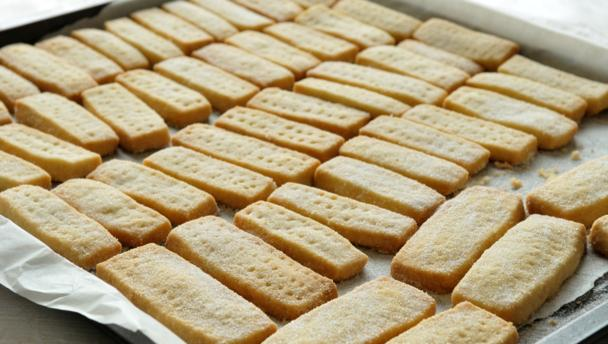
\includegraphics[width=8cm]{shortbread}
\caption{this is a picture of shortbread}
\end{figure}


\chapter{Liam Scarlett}
\section{Spinach, feta and broad bean pie}
This fabulous vegetarian pie contains broad beans, fetta cheese and spinach in a crunchy wholemeal pastry.
\section{Ingredients:}
\begin{itemize}
	\item 2 cups wholemeal plain flour
	\item 1 cup wheatgerm
	\item 160g butter, chilled, chopped
	\item 4 eggs
	\item 2 tablespoons chilled water
	\item 2 teaspoons olive oil
	\item 1 large brown onion, finely chopped
	\item 2 garlic cloves, crushed
	\item 200g baby spinach
	\item 2 cups (300g) fresh broad beans
	\item 100g feta, crumbed
	\item 2 tablespoons finely grates hard cheese or parmesan
	\item 1 tablespoon chopped fresh dill
	\item 1 teaspoon finely grated lemon rind
	\item 1/3 cup milk
\end{itemize}

\section{Instructions:}
\begin{enumerate}
\item Place flour, wheatgerm and butter in a food processor. Process until mixture resembles fine breadcrumbs. Add 1 egg and chilled water. Process until mixture just comes together and forms a soft dough, adding extra water if necessary. Turn out onto a lightly floured surface. Knead until smooth. Shape into a disc. Wrap in plastic wrap. Refrigerate 30 minutes or until firm.
\item Meanwhile, heat oil in a large, deep frying pan over medium-high heat. Add onion. Cook for 5 minutes or until softened. Add garlic. Cook, stirring, for 1 minute or until fragrant. Add spinach. Cook for 2 minutes or until wilted. Transfer mixture to a colander over a bowl to strain. Cool for 10 minutes.
\item Place broad beans in a heatproof bowl. Cover with boiling water. Set aside for 30 seconds. Drain. Refresh in a bowl of chilled water. Drain. Peel and discard skins.
\item Preheat oven to 190C/170C fan-forced. Roll pastry out between 2 sheets of baking paper until 5mm thick. Line a 4cm-deep, 22cm (top) pie plate with pastry. Trim excess. Pinch edge of pastry to form a decorative pattern.
\item Place spinach mixture in a bowl. Add broad beans, fetta, cheese, dill and lemon rind. Whisk milk and remaining eggs together. Add to broad bean mixture. Season with salt and pepper. Stir until well combined. Spoon mixture into pastry case. Place on a baking tray. Bake for 45 minutes or until golden and filling has set. Stand for 10 minutes. Cut into wedges. Serve.
\end{enumerate}


\chapter{Erica Thygesen}
\section{Panna cotta}

\section{Ingredients}
\begin{itemize}
        \item 500ml thickened cream
        \item 150ml whole milk
        \item 180g caster sugar
	\item 1 vanilla pod
	\item 3 leaves gold leaf gelatine
	\item Berries, to serve
\end{itemize}

\section{Method}

\begin{enumerate}
\item Place the cream, milk, sugar, and scraped vanilla beans and pod in a large pan. Stir over a low-medium heat and slowly bring to the boil. When the mixture just reaches the boil, remove from the heat immediately.
\item Meanwhile, place the gelatin leaves in a shallow dish, and then cover in cold water to soften for 5 minutes. Remove the gelatin from the water and squeeze out any excess water. Whisk the gelatin into to the cream mixture until dissolved.
\item Allow the mixture to cool slightly and then strain through a sieve into a jug. Pour into 6x120ml capacity pudding moulds, and then transfer into the refrigerator for 5 hours or until set. The panna cottas should still have a slight wobble to them once set.
\item Remove the panna cottas from the fridge and run a sharp knife around the edge of the moulds. Dip the moulds briefly into hot water and then use your fingers to gently loosen the panna cottas away from the edges. Turn upside down to release the panna cottas from the moulds.
\item Serve the panna cottas immediately with berries. 
\end{enumerate}



\chapter{Ivan Lau}
\section{My Biography}
Ivan Lau biography for the Pawsey Supercomputing Centre Summer Internship

\subsection{About Me}
I am a third year Medical Imaging student from Curtin University and just about to enter my exciting final year next year. The project that I will be working on in this internship will be about determining the clinical value of realistic 3D printed heart models in helping physicians to understand patient-specific cardiovascular pathology and thus improving the presurgical planning in congenital heart diseases. 
I am hoping to gain experience and develop skills in planning and conducting scientific and academic research, and more importantly, I am excited to see how the programming skills and supercomputers can help me to conduct a much better and faster research.




\chapter{Ozlem Erkilic}
/section{My biography}
Ozlem Erkilic's Biography for Pawsey Supercomputing Centre

/subsection{!about Ozlem }
I am Ozlem Erkilic. I study Physics and Electronic and Communication
Engineering at Curtin University. I just finished the third year of my degree
and still have 2 more years to graduate.
My internship project involves writing scripts for the use of supercomputers
and developing a tool called getexample which includes sample codes to help
researches to perform particular tasks on supercomputers. 


\chapter{Nicholas Lawler}
\section{My Biography}

Nicholas Lawler's biography for the Pawsey Supercomputing Centre Summer Internship

\subsection{About me}
I am a second year Bachelor of Philosophy (Honours) student from UWA, majoring in Physics and Engineering.
I am working with Professor Kenji Bekki from ICRAR to explore galaxy transformation from early- to late-types. This involves the investigatation of which physical conditions of `E-Sp’ merging result in the formation of a new disk galaxy. The simulated distributions and kinematics of gas and stars will be compared with corresponding observations of disk galaxies.



\end{document}

